\chapter{Part 3}

\section{Introduction}
%• Very brief introduction of the overall problem setting (< page
%max)

Now describe the setup for the FlexRay modeling part, Figure \ref{fig:FRdia} shows the most important given parts and also the tree view in Inchron along with the FlexRay bus connections.

\begin{figure}[h!]
	\begin{center}
		
			\begin{tabular}{cc}
				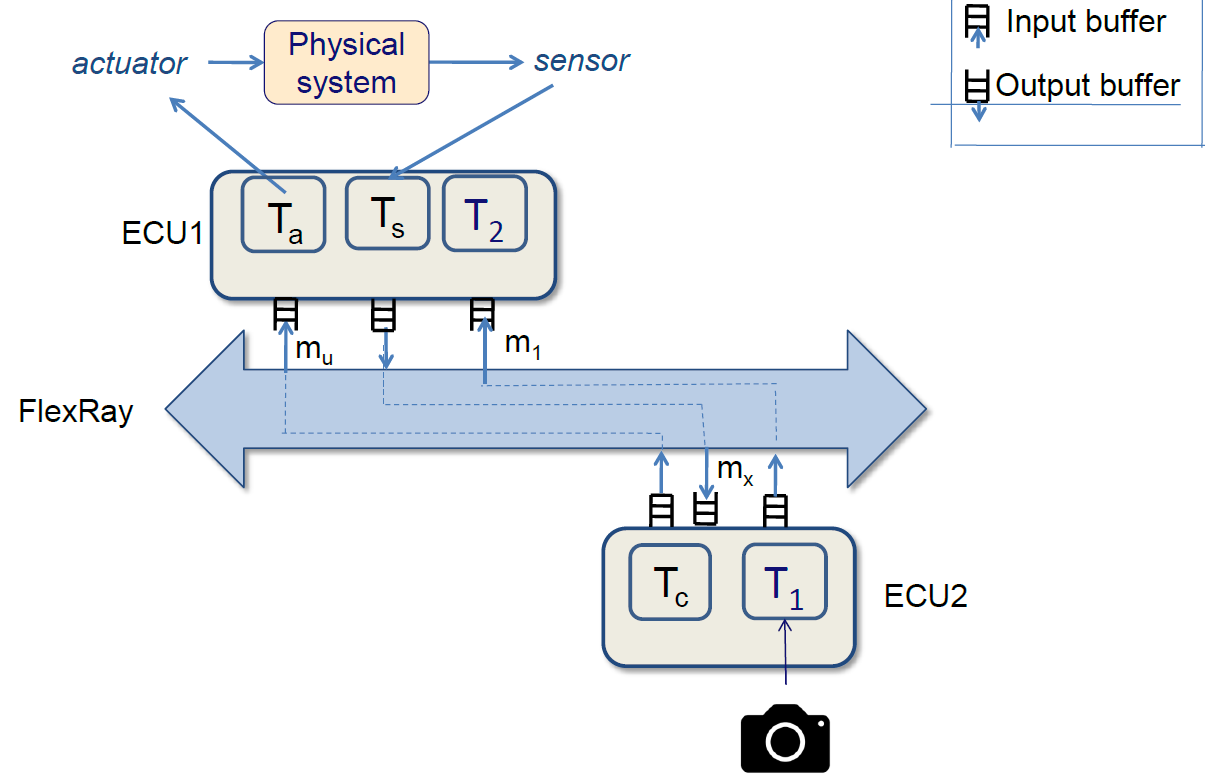
\includegraphics[width=0.5\linewidth]{img/FR-diagram} & 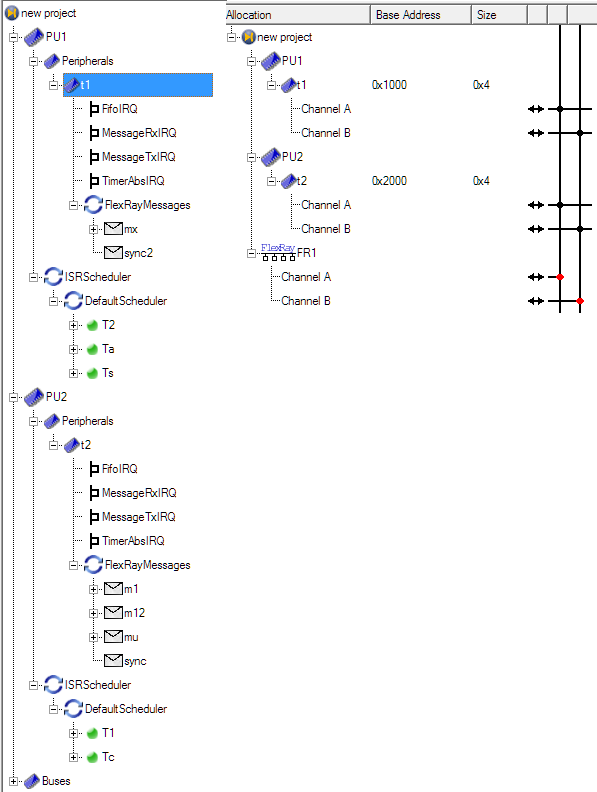
\includegraphics[width=0.35\linewidth]{img/FR-setup}	\\
			\end{tabular}
			\caption{On the left, system diagram and on the right the tree view and architecture of the Inchron project. }
		\caption{}
		\label{fig:FRdia}
	\end{center}
\end{figure}


\section{Answer all the questions}

\subsection{Theoretical analysis versus actual implementation}
%Comment on differences from the theoretical analysis and actual implementation


\section{Design decision}
%• Your design decision and justification.

\section{Results}

Firstly: Solution to the design problem. (Include the parameters you have chosen)\\
Secondly: from chronVIEW for your design

\section{Conclusions}